\documentclass{beamer}

\usetheme[progressbar=frametitle]{metropolis}
\usepackage{appendixnumberbeamer}
\usepackage{booktabs}
\usepackage{amsmath}
\usepackage{amssymb}
\usepackage{tcolorbox}
\usepackage{tikz}

\definecolor{metropolisblue}{RGB}{39, 59, 94}



% Begin document
\begin{document}

% Title page
\title{Sampling Methods}
\author{Nipun Batra}
\date{\today}
\institute{IIT Gandhinagar}
\maketitle

\begin{frame}{Topics}
    %TOC with enumerated items
    \setbeamertemplate{section in toc}[sections numbered]
    \tableofcontents

\end{frame}

\begin{frame}{Main Goal}
    \begin{itemize}
        \item We want to compute posterior predictive distribution (or something similar)
        \pause \item We would typically use Monte Carlo methods to do this.
        \pause \item $I = \int f(x) p(x) dx$ where $p(x)$ is the posterior distribution.
        \pause \item We can approximate $I$ by $\frac{1}{N} \sum_{i=1}^N f(x_i)$, where $x_i \sim p(x)$.
        \pause \item Goal: sample from $p(x)$.
    \end{itemize}
\end{frame}

\subsection{Rejection Sampling}
    \begin{frame}{Rejection Sampling}
        \begin{itemize}
            \item Let $p(x)$ be the target distribution from which we want to sample.
            \pause \item Typically, $p(x)$ is the posterior distribution.
            \pause \item But, we do not have access to $p(x)$. Rather, we have access to $\tilde{p}(x)$, which is proportional to $p(x)$.
            \pause \item We can write $p(x) = \frac{\tilde{p}(x)}{Z}$, where $Z$ is the normalization constant.
            \pause \item Typically, $\tilde{p}(x)$ is the joint distribution of the data and the parameters.
            \pause \item Let $q(x)$ be a proposal distribution from which we can sample.
            \pause \item Let $M$ be a constant such that $M \geq \frac{\tilde{p(x)}}{q(x)}$ for all $x$.
            \pause \item Then, we can sample from $p(x)$ by sampling from $q(x)$ and accepting the sample with probability $\frac{p(x)}{M q(x)}$.
        \end{itemize}
        
    \end{frame}

    \begin{frame}
        Notebook: \url{rejection-sampling.ipynb}
    \end{frame}

   \begin{frame}{Rejection Sampling}
    \begin{figure}
        \centering
        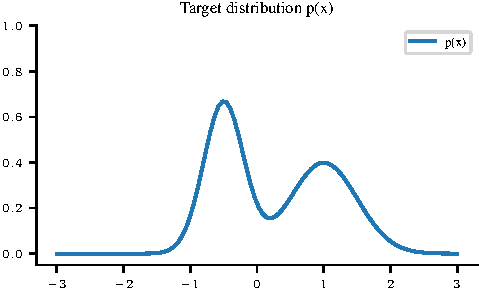
\includegraphics[scale = 0.75]{../figures/sampling/rejection-sampling--1.0-False-False-False-False-False-False-False-False.pdf}
    \end{figure}
    
   \end{frame}

    \begin{frame}{Rejection Sampling}
        \begin{figure}
            \centering
            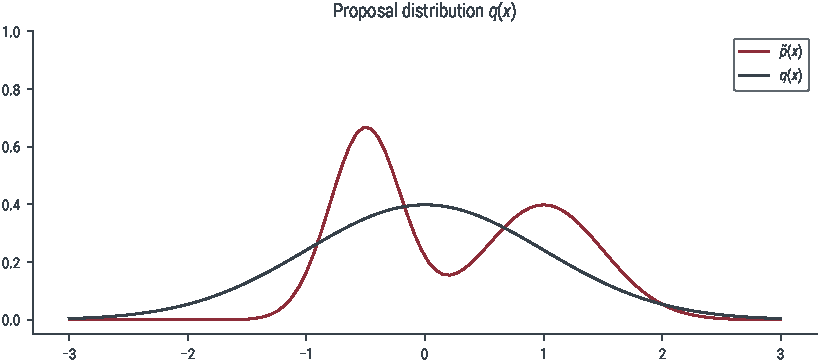
\includegraphics[scale = 0.75]{../figures/sampling/rejection-sampling--1.0-True-False-False-False-False-False-False-False.pdf}
        \end{figure}
    \end{frame}

    \begin{frame}{Rejection Sampling}
        \begin{figure}
            \centering
            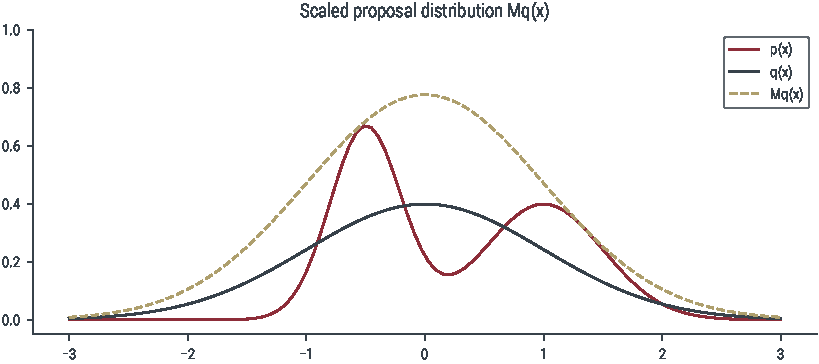
\includegraphics[scale = 0.75]{../figures/sampling/rejection-sampling--1.0-True-True-False-False-False-False-False-False.pdf}
        \end{figure}
    \end{frame}

    \begin{frame}{Rejection Sampling}
        \begin{figure}
            \centering
            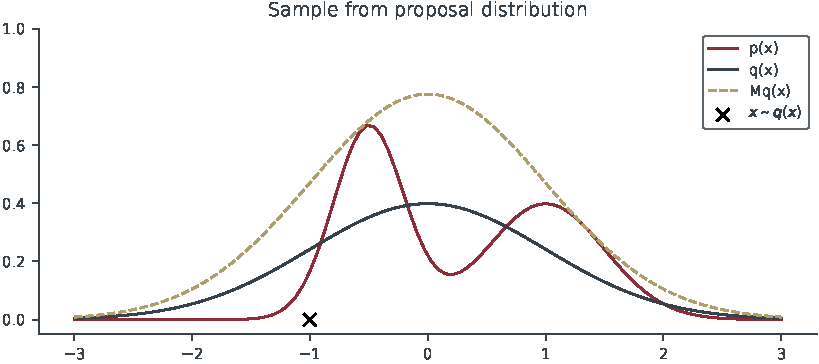
\includegraphics[scale = 0.75]{../figures/sampling/rejection-sampling--1.0-True-True-True-False-False-False-False-False.pdf}
        \end{figure}
    \end{frame}

    \begin{frame}{Rejection Sampling}
        \begin{figure}
            \centering
            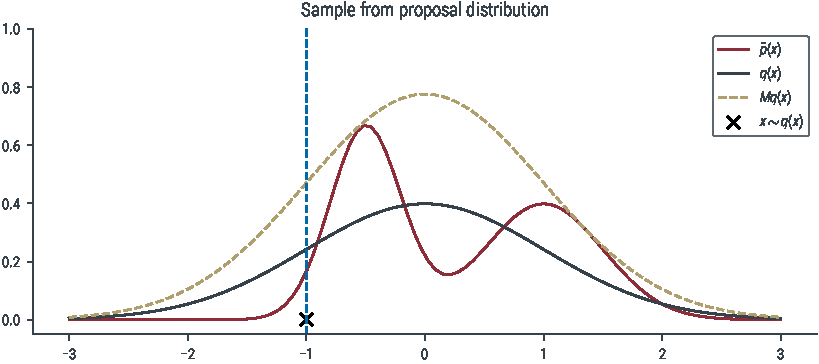
\includegraphics[scale = 0.75]{../figures/sampling/rejection-sampling--1.0-True-True-True-True-False-False-False-False.pdf}
        \end{figure}
    \end{frame}

    \begin{frame}{Rejection Sampling}
        \begin{figure}
            \centering
            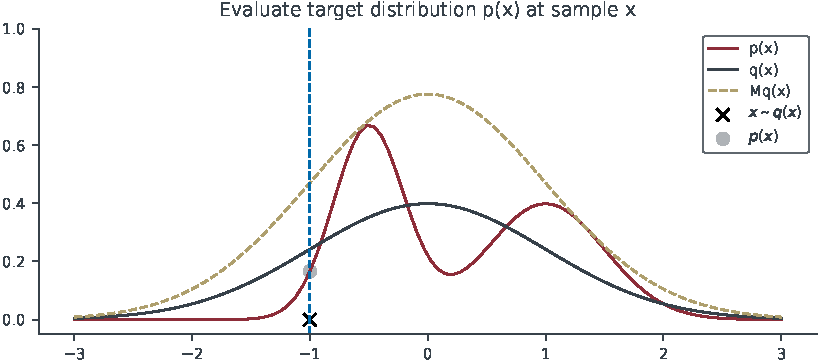
\includegraphics[scale = 0.75]{../figures/sampling/rejection-sampling--1.0-True-True-True-True-True-False-False-False.pdf}
        \end{figure}
    \end{frame}

    \begin{frame}{Rejection Sampling}
        \begin{figure}
            \centering
            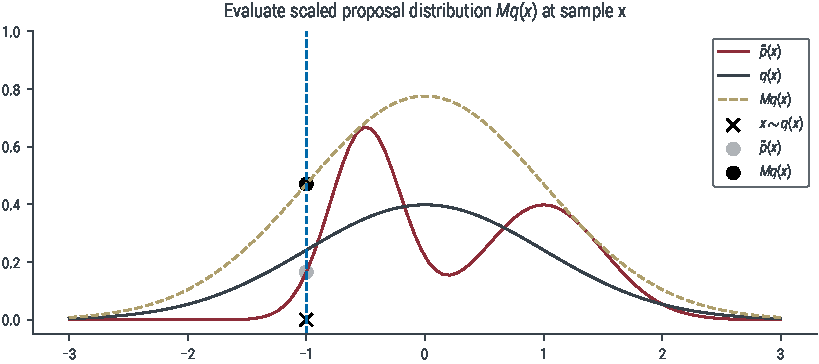
\includegraphics[scale = 0.75]{../figures/sampling/rejection-sampling--1.0-True-True-True-True-True-True-False-False.pdf}
        \end{figure}
    \end{frame}

    \begin{frame}{Rejection Sampling}
        \begin{figure}
            \centering
            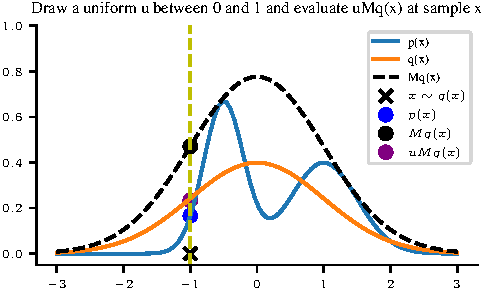
\includegraphics[scale = 0.75]{../figures/sampling/rejection-sampling--1.0-True-True-True-True-True-True-True-False.pdf}
        \end{figure}
    \end{frame}

    \begin{frame}{Rejection Sampling (Rejected Sample)}
        \begin{figure}
            \centering
            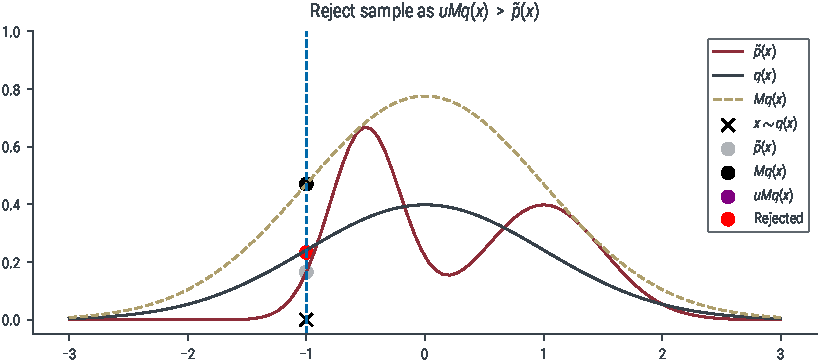
\includegraphics[scale = 0.75]{../figures/sampling/rejection-sampling--1.0-True-True-True-True-True-True-True-True.pdf}
        \end{figure}
    \end{frame}


    \begin{frame}{Rejection Sampling (Accepted Sample)}
        \begin{figure}
            \centering
            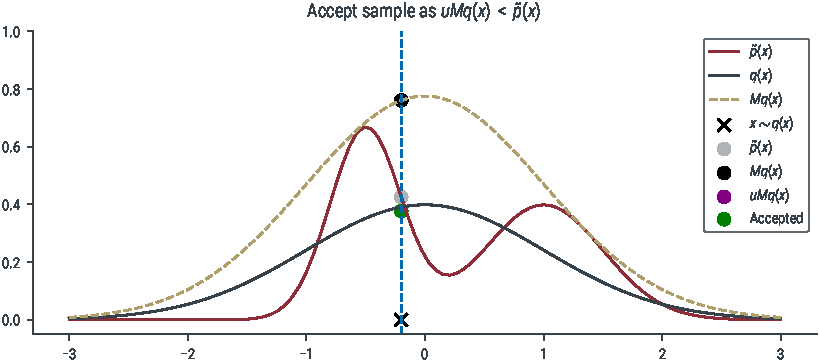
\includegraphics[scale = 0.75]{../figures/sampling/rejection-sampling--0.2-True-True-True-True-True-True-True-True.pdf}
        \end{figure}
    \end{frame}

    \foreach \n in {10, 1000, 10000}{
    \begin{frame}{Rejection Sampling (\n{} samples)}
        \includegraphics[width=\textwidth]{../figures/sampling/rejection-sampling-N\n-False.pdf}
    \end{frame}

    \begin{frame}{Rejection Sampling (\n{} samples) (KDE)}
        \includegraphics[width=\textwidth]{../figures/sampling/rejection-sampling-N\n-True.pdf}
    \end{frame}
}

\begin{frame}{Rejection Sampling Proof}
    \begin{itemize}
        \item Acknowledgement: Borrowed from ritvikmath YT channel
        \item Aim: 
        \begin{itemize}
            \pause \item Show that the samples we accept are distributed according to $p(x)$. 
            \pause \item Or, the density of an accepted sample (say $x_s$) is $p(x_s)$ (and not $\tilde{p}(x_s)$).
        \end{itemize}
           

            \pause \item Acceptance Probability $\alpha(x)$: Probability that we accept a sample $x_s$ generated from $q(x)$.
        \begin{equation}
            \alpha(x_s) = \frac{\tilde{p}(x_s)}{M q(x_s)} = P(Accept|x_s)
        \end{equation}

        
    \end{itemize}
\end{frame}

\begin{frame}{Rejection Sampling Proof}
    
    \begin{itemize}
        
        \item Bayes Rule for Acceptance:
        \begin{equation}
            P(x_s|Accept) = \frac{P(Accept|x_s) P(x_s)}{P(Accept)}
        \end{equation}
        
        \begin{itemize}
           
        
        \item where $P(x_s|Accept)$ is the density of accepted sample $x_s$. We want to evaluate this and show this is $p(x_s)$.
        
        \pause
        
        \item $P(Accept|x_s)$ is $\alpha(x_s)$
        
        \pause
        \item $P(x_s) = q(x)$ is the density of samples we draw from $q(x)$.
        
        \pause 
        \item $P(Accept)$ is the unconditional probability that we accept a sample generated from $q(x)$.
    \end{itemize}

    \end{itemize}
    
    
\end{frame}


\begin{frame}{Proof of Rejection Sampling}

\begin{itemize}
    \item  P(Accept) is the unconditional probability that we accept a sample generated from $q(x)$.
    \pause \begin{equation}
        P(Accept) = \int P(Accept|x_s) P(x_s) dx_s
    \end{equation}

    \pause \begin{equation}
        P(Accept) = \int \alpha(x_s) q(x_s) dx_s
    \end{equation}
    
    \pause \begin{equation}
        P(Accept) = \int \frac{\tilde{p}(x_s)}{M q(x_s)} q(x_s) dx_s
    \end{equation}

    \pause \begin{equation}
        P(Accept) = \frac{1}{M} \int \tilde{p}(x_s) dx_s
    \end{equation}

    \pause \begin{equation}
        P(Accept) = \frac{Z}{M}
    \end{equation}

    where $Z$ is the normalization constant of $\tilde{p}(x)$.
\end{itemize}
    
\end{frame}

\begin{frame}{Proof of Rejection Sampling}
    Plugging in the values

    \begin{equation}
        P(x_s|Accept) = \frac{P(Accept|x_s) P(x_s)}{P(Accept)}
    \end{equation}

    \pause \begin{equation}
        P(x_s|Accept) = \frac{\alpha(x_s) q(x_s)}{P(Accept)}
    \end{equation}

    \pause \begin{equation}
        P(x_s|Accept) = \frac{\frac{\tilde{p}(x_s)}{M q(x_s)} q(x_s)}{\frac{Z}{M}}
    \end{equation}

    \pause \begin{equation}
        P(x_s|Accept) = \frac{\tilde{p}(x_s)}{Z}
    \end{equation}

    \pause \begin{equation}
        P(x_s|Accept) = p(x_s)
    \end{equation}

    
\end{frame}

\begin{frame}{Thought Experiment}
    \begin{itemize}
        \item Let us assume $\tilde{p}(x)$ is $D$ dimensional Gaussian $\mathcal{N}_D(0, \sigma_p^2 I)$
        \pause \item Let us assume our proposal distribution $q(x)$ is $\mathcal{N}_D(0, \sigma_q^2 I)$
        \pause 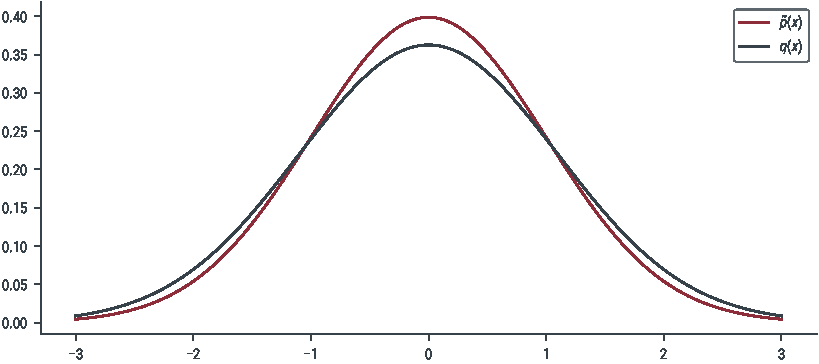
\includegraphics[width=\textwidth]{../figures/sampling/rejection-sampling-gaussian-p-q.pdf}
        \item How to choose multiplier $M$?
        \item Match the densities at the peak of $\tilde{p}(x)$ and $q(x)$, i.e. at $x = \vec{0}$.
    \end{itemize}

    
\end{frame}

\begin{frame}{Thought Experiment}
    \begin{itemize}
        \item Match the densities at the peak of $\tilde{p}(x)$ and $q(x)$, i.e. at $x = \vec{0}$.
        \pause \item $\tilde{p}(x) = \frac{1}{(2\pi)^{D/2} \sigma_p^D} \exp(-\frac{1}{2\sigma_p^2} x^T x)$
        \pause \item $q(x) = \frac{1}{(2\pi)^{D/2} \sigma_q^D} \exp(-\frac{1}{2\sigma_q^2} x^T x)$
        \pause \item At $x = \vec{0}$, $\tilde{p}(x) = \frac{1}{(2\pi)^{D/2} \sigma_p^D}$ and $q(x) = \frac{1}{(2\pi)^{D/2} \sigma_q^D}$
        \pause \item $M = \frac{\tilde{p}(x)}{q(x)} = \frac{\sigma_q^D}{\sigma_p^D} = (\frac{\sigma_q}{\sigma_p})^D$
    \end{itemize}

    
\end{frame}

\begin{frame}{Thought Experiment}
    \begin{itemize}
        \item $M = \frac{\tilde{p}(x)}{q(x)} = \frac{\sigma_q^D}{\sigma_p^D} = (\frac{\sigma_q}{\sigma_p})^D$
        \item Let us assume $\sigma_p = 1$ and $\sigma_q = 1.1$
    \end{itemize}
    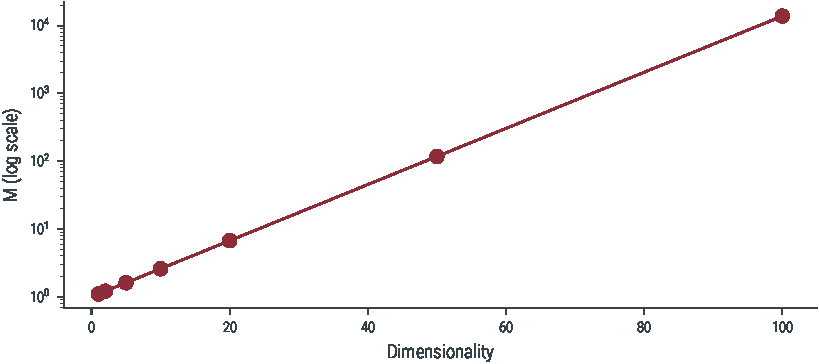
\includegraphics[width=\textwidth]{../figures/sampling/rejection-sampling-gaussian-p-q-M.pdf}

    
\end{frame}
   
\begin{frame}{Thought Experiment}
    \begin{itemize}
        \item $M = \frac{\tilde{p}(x)}{q(x)} = \frac{\sigma_q^D}{\sigma_p^D} = (\frac{\sigma_q}{\sigma_p})^D$
        \item Let us assume $\sigma_p = 1$ and $\sigma_q = 1.1$
       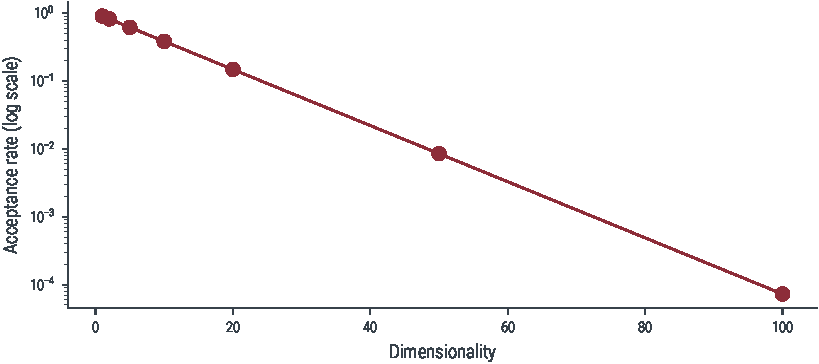
\includegraphics[width=\textwidth]{../figures/sampling/rejection-sampling-gaussian-p-q-acceptance.pdf}
        \item Acceptance probability is very low as $D$ increases.
    \end{itemize}

    
\end{frame}
    

    \begin{frame}{Challenges with Rejection Sampling}
        \begin{itemize}
            \item Rejection sampling is inefficient when the target distribution is very different from the proposal distribution. In this case, we will reject a lot of samples.
            \item This is a problem when sampling from high-dimensional distributions. Acceptance probability $\alpha(x)$ is very low.
        \end{itemize}
    \end{frame}

\subsection{Importance Sampling}

\begin{frame}{Back to the main problem at hand}
    \begin{itemize}
        \item We want to compute posterior predictive distribution (or something similar)
        \item We would typically use Monte Carlo methods to do this.
        \item $I = \int f(x) p(x) dx$ where $p(x)$ is the posterior distribution.
        \item We can approximate $I$ by $\frac{1}{N} \sum_{i=1}^N f(x_i)$, where $x_i \sim p(x)$.
        \item But, we do not have access to $p(x)$. Rather, we have access to $\tilde{p}(x)$, which is proportional to $p(x)$.
    \end{itemize}
    
\end{frame}

\begin{frame}{Back to the main problem at hand}
    \begin{itemize}
        \item We can approximate $I$ by $\frac{1}{N} \sum_{i=1}^N f(x_i)$, where $x_i \sim p(x)$.
        \item But, we do not have access to $p(x)$. Rather, we have access to $\tilde{p}(x)$, which is proportional to $p(x)$.
        \item In rejection sampling, we took a sample $x_i$ from $q(x)$ and accepted it with probability $\frac{\tilde{p}(x_i)}{M q(x_i)}$.
        \item Can we use all samples $x_i$ from $q(x)$ without rejection?
    \end{itemize}
    
\end{frame}

\begin{frame}{Importance Sampling}
    \begin{itemize}
        \item In rejection sampling, we took a sample $x_i$ from $q(x)$ and accepted it with probability $\frac{\tilde{p}(x_i)}{M q(x_i)}$.
        \item Can we use all samples $x_i$ from $q(x)$ without rejection?
        \item $I = \int f(x) p(x) dx \approx \frac{1}{N} \sum_{i=1}^N f(x_i)$, where $x_i \sim p(x)$.
        \item Let us choose a proposal distribution $q(x)$ which has support over the entire domain of $p(x)$.
        \item $I = \int f(x) p(x) dx = \int f(x) \frac{p(x)}{q(x)} q(x) dx$
        \item $I = \int f(x) w(x) q(x) dx$, where $w(x) = \frac{p(x)}{q(x)}$. $w(x)$ is called the importance weight.
        \item $I = \mathbb{E}_q[f(x) w(x)] = \sum_{i=1}^N f(x_i) w(x_i)$, where $x_i \sim q(x)$.
    \end{itemize}
    
\end{frame}

\begin{frame}{Importance Sampling (with unnormlized $\tilde{p}(x)$ instead of $p(x)$)}
    \begin{equation}
        \begin{aligned}
        I = \int f(x) p(x) \mathrm{d} x & \approx \frac{1}{Z} \frac{1}{S} \sum_s f\left(x_S\right) \frac{\tilde{p}\left(x_S\right)}{q\left(x_S\right)} \\
        \end{aligned}
        \end{equation}

        Now, we need to estimate $Z$.

        \begin{equation}
        \begin{aligned}
        Z &= \int \tilde{p}(x) \mathrm{d} x &= \int \frac{\tilde{p}(x)}{q(x)} q(x) \mathrm{d} x \\
        &= \mathbb{E}_q \left[ \frac{\tilde{p}(x)}{q(x)} \right] &= \frac{1}{S} \sum_s \frac{\tilde{p}\left(x_S\right)}{q\left(x_S\right)}
        \end{aligned}
        \end{equation}

        Thus, we can write $I$ as:
        \begin{equation}
        \begin{aligned}
            I  \approx \frac{1}{S} \sum_s f\left(x_s\right) \frac{\tilde{p}\left(x_s\right) / q\left(x_s\right)}{\frac{1}{s} \sum_t \tilde{p}\left(x_t\right) / q\left(x_t\right)}=: \sum_s f\left(x_s\right) \tilde{w}_s
            \end{aligned}
        \end{equation}
\end{frame}


\section{Markov Chains}
\begin{frame}
    \url{https://nipunbatra.github.io/hmm/}
\end{frame}

\begin{frame}{Global Optimization}
    Notebook: mcmc=optimization.ipynb
    
\end{frame}


\begin{section}{Importance Sampling}
    \begin{frame}{General Form}
        In rejection sampling, we saw that due to less acceptance probability, a lot of samples were wasted leading to more time and higher complexity to approximate a distribution.

        Computing $p(x), q(x)$ thus seems wasteful. Let us rewrite the equation as:
        \begin{align*}
            \phi &= \int f(x)p(x)dx = \int f(x)\frac{p(x)}{q(x)}q(x)dx \\
            &\sim \frac{1}{N} \sum_{i=1}^Nf(x_i)\frac{p(x_i)}{q(x_i)} = \frac{1}{N} \sum_{i=1}^Nf(x_i)w_i 
        \end{align*}
        Here, $x_i\sim q(x)$. $w_i$ is known as the importance(weight) of sample i. 
    \end{frame}

    \begin{frame}
        However the normalization constant $Z$ is generally not known to us. Thus writing: 
        \begin{equation}
            p(x) = \frac{\Tilde{p}(x)}{Z}
        \end{equation}
        Now inserting this in earlier equations, we get:
        \begin{align*}
            \phi &=\frac{1}{Z} \int f(x)\Tilde{p}(x)dx = \frac{1}{Z}\int f(x)\frac{\Tilde{p}(x)}{q(x)}q(x)dx \\
            &\sim \frac{1}{NZ} \sum_{i=1}^Nf(x_i)\frac{\Tilde{p}(x_i)}{q(x_i)} = \frac{1}{NZ} \sum_{i=1}^Nf(x_i)w_i 
        \end{align*}
        We know that:
        \begin{align*}
            Z &= \int_{\infty}^{\infty} \Tilde{p}(x)dx = \int_{\infty}^{\infty}\frac{\Tilde{p}(x)}{q(x)}q(x)dx \\
            &= \frac{1}{N}\sum_{i=1}^N w_i
        \end{align*}
    \end{frame}

    \begin{frame}
        Substuting this value of $Z$ in the equation above, we get:
        \begin{align*}
            \phi &= \frac{1}{N}\sum_{i=1}^N f(x_i)w_i = \frac{\sum_{i=1}^N f(x_i)w_i}{\sum_{i=1}^N w_i} \\
            &= \sum_{i=1}^N f(x_i)W_i
        \end{align*}
        Here $W_i = \frac{w_i}{\sum_{i=1}^N w_i}$ are the normalized weights.
    \end{frame}

    \begin{frame}{Limitations}
        \begin{itemize}
            \item Recall that Var $\hat{\phi} = \frac{var(f)}{N}$. Importance sampling replaces $var(f)$ with $var(f\frac{p}{q})$. At positions where $p>>>q$, the weight can tend to $\infty$!
        \end{itemize}
        \begin{figure}
                \centering
                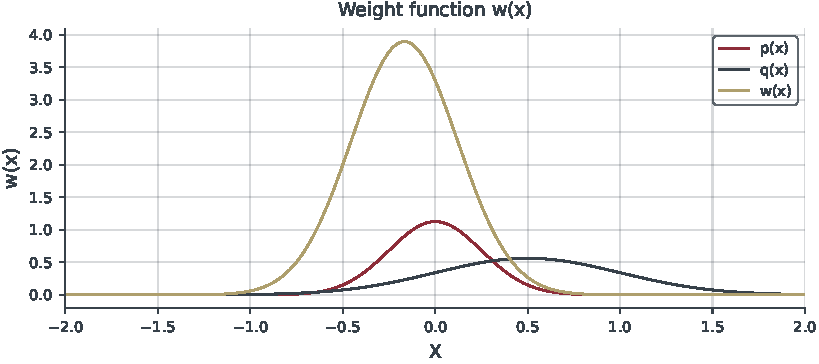
\includegraphics[scale=0.8]{../figures/importance_sampling_weight_function.pdf}
        \end{figure}
    \end{frame}
\end{section}

\begin{section}{Gibbs Sampling}
    \begin{frame}{General Form}
        Suppose we wish to sample $\theta_1, \theta_2 \sim p(\theta_1, \theta_2)$, but cannot use:\\
        \begin{itemize}
            \item direct simulation
            \item accept-reject method
            \item Metropolis-Hasting
        \end{itemize}
        But we can sample using the conditionals i.e.:\\
        \begin{itemize}
            \item $p(\theta_1|\theta_2)$ and
            \item $p(\theta_2|\theta_1)$,
        \end{itemize}
        then we can use Gibbs sampling.
    \end{frame}
    
    \begin{frame}
        Suppose $\theta_1, \theta_2 \sim p(\theta_1, \theta_2)$ and we can sample from $p(\theta_1, \theta_2)$. We begin with an initial value $(\theta_1^{0}, \theta_2^{0})$, the workflow for Gibbs algorithm is:\\
        1. sample $\theta_1^j \sim p(\theta_1|\theta_2^{j-1})$ and then\\
        2. sample $\theta_2^j \sim p(\theta_2|\theta_1^j)$.\\
        One thing to note here is that the sequence in which the theta's are sampled are not independent!    
    \end{frame}

    \begin{frame}{Bivariate Normal Example}
        Suppose \\
        $\theta \sim N_2(0,\Sigma)$ and $\Sigma = $
        $ \begin{matrix}
        1 & \rho \\
        \rho & 1  
        \end{matrix} $
    
    Then, we have:\\
    $\theta_1|\theta_2 \sim N(\rho\theta_2,[1-\rho^2])$

    $\theta_2|\theta_1 \sim N(\rho\theta_1,[1-\rho^2])$
    are the conditional distributions.
    The Gibbs sampling proceeds as follows:\\
    \begin{table}[]
        \centering
        \begin{tabular}{c c c}
           Iteration & Sample $\theta_1$ & Sample $\theta_2$\\
           \hline
           1  &  $\theta_1\sim N(\rho\theta_2^0, [1-\rho^2])$ &  $\theta_2\sim N(\rho\theta_1^1, [1-\rho^2])$\\
           & . & \\
           & . & \\
           $k$  &  $\theta_1\sim N(\rho\theta_2^{k-1}, [1-\rho^2])$ &  $\theta_2\sim N(\rho\theta_1^k, [1-\rho^2])$
             
        \end{tabular}
    \end{table}
    \end{frame}

    \begin{frame}
        \begin{figure}
                \centering
                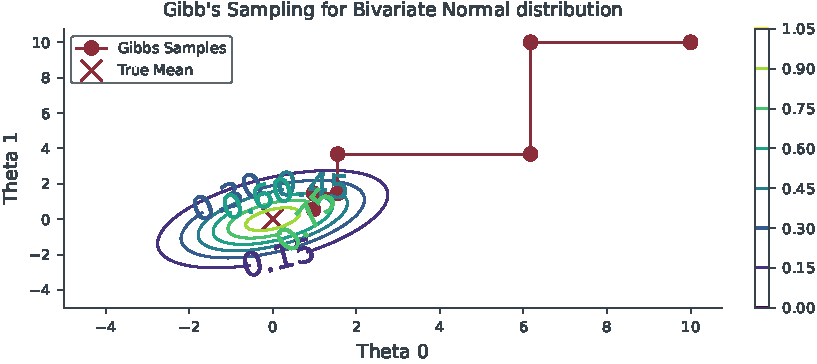
\includegraphics[scale=0.8]{../figures/gibbs_sampling_bivariate_normal.pdf}
            \end{figure}
    \end{frame}

    \begin{frame}{Multivariate case}
        Suppose $\theta = (\theta_1, \theta_2, \ldots, \theta_K)$, the Gibbs workflow is as follows:\\
        $\theta_1^j = p(\theta_1|\theta_2^{j-1}, \ldots, \theta_K^{j-1})$\\
        $\theta_2^j = p(\theta_2|\theta_1^{j}, \theta_3^{j-1}, \ldots, \theta_K^{j-1})$\\
        .\\
        .\\
        $\theta_k^j = p(\theta_k|\theta_1^{j}, \ldots, \theta_{k-1}^j, \theta_{k+1}^{j-1}, \ldots, \theta_K^{j-1})$\\
        .\\
        .\\
        $\theta_K^j = p(\theta_K|\theta_1^{j}, \ldots, \theta_{K-1}^{j})$\\
        The distributions above are call the full conditional distributions.
    \end{frame}

    \begin{frame}{Advantages}
        Gibbs sampling can be used to draw samples from $p(\theta)$ when:\\
        \begin{itemize}
            \item Other methods don't work quite well in higher dimensions.
            \item Draw samples from the full conditional distributions is easy, $p(\theta_k|\theta_{-k}).$
        \end{itemize}
    \end{frame}
\end{section}

\begin{section}{Markov Chain Monte Carlo}
    \begin{frame}{Limitations of basic sampling methods}
        \begin{itemize}
            \item \textit{Transformation based methods}: Usually limited to drawing from standard distributions.
            \item \textit{Rejection and Importance sampling}: Require selection of good proposal distirbutions.
        \end{itemize}
        In high dimensions, usually most of the density $p(x)$ is concentrated within a tiny subspace of $x$. Moreover, those subspaces are difficult to be known a priori.

        A solution to these are MCMC methods.
    \end{frame}

    \begin{frame}{Markov Chain}
        \begin{itemize}
            \item \textbf{Markov Chain}: A joint distribution $p(X)$ over a sequence of random variables $X = \{X_1, X_2, \ldots, X_n\}$ is said to have the Markov property if 
            $$
            p(X_i|X_1, \ldots, X_{i-1}) = p(X_i|X_{i-1}) 
            $$
            The sequence is then called a Markov chain.
            \item The idea is that the estimates contain information about the shape of the target distribution $p$.
        \end{itemize}
    \end{frame}

    \begin{frame}{Metropolis Hastings}
        \begin{itemize}
            \item The basic idea is propose to move to a new state $x_{i+1}$ from the current state $x_i$ with probability $q(x_{i+1}|x_i)$, where $q$ is called the proposal distribution and our target density of interest is $p (= \frac{1}{Z} \tilde{p})$.
            \item The new state is accepted with probability $\alpha(x_i, x_{i+1})$.
            \begin{itemize}
                \item If $p(x_{i+1}| x_i) = p(x_i| x_{i+1})$, then $\alpha(x_i, x_{i+1}) = \min (1, \frac{p(x_{i+1})}{p(x_i)})$.
                \item If $p(x_{i+1}| x_i) \neq p(x_i| x_{i+1})$, then $\alpha(x_i, x_{i+1}) = \min (1, \frac{p(x_{i+1})q(x_i|x_{i+1})}{p(x_i)q(x_{i+1}|x_i)}) = \min (1, \frac{\tilde{p}(x_{i+1})q(x_i|x_{i+1})}{\tilde{p}(x_i)q(x_{i+1}|x_i)})$
            \end{itemize}
            \item Evaluating $\alpha$, we only need to know the target distribution up to a constant of proportionality or without normalization constant.
        \end{itemize}
    \end{frame}

    \begin{frame}{Algorithm: Metropolis Hastings}
        \begin{enumerate}
            \item Initialize $x_0$.
            \item for $i = 1, \ldots, N$ do:
            \item \quad Sample $x^* \sim q(x^*|x_{i-1})$.
            \item \quad Compute $\alpha = \min (1, \frac{\tilde{p}(x^*)q(x_{i-1}|x^*)}{\tilde{p}(x_{i-1})q(x^*|x_{i-1})})$
            \item \quad Sample $u \sim \mathcal{U}(0, 1)$
            \item \quad if $u \leq \alpha$:
            
            \quad \quad $x_i = x^*$
            
            \quad else:
            
            \quad \quad $x_i = x_{i-1}$
        \end{enumerate}
    \end{frame}

    \begin{frame}{Pop Quiz}
        How do we choose the initial state $x_0$?
        \pause
        \begin{enumerate}
            \item Start the Markov Chain at an initial $x_0$.
            \item Using the proposal $q(x|x_i)$, run the chain long enough, say $N_1$ steps.
            \item Discard the first $N_1 - 1$ samples (called 'burn-in' samples).
            \item Treat $x_{N_1}$ as first sample from $p(x)$.
        \end{enumerate}
    \end{frame}

    \begin{frame}{MCMC demo}
        
        \url{https://chi-feng.github.io/mcmc-demo/app.html}
    \end{frame}
\end{section}

\end{document}